\documentclass{beamer}
\usepackage{etex}


\usepackage{multicol}
\usepackage{calc}
\usepackage{ifthen}
\usepackage{beamerthemeshadow}
\setbeamertemplate{navigation symbols}{}
%packages indispensables 
\usepackage[utf8]{inputenc}
\usepackage{lmodern}
\usepackage{graphicx}
%packages utiles
\usepackage{alltt} %program code
\usepackage{enumerate}
\usepackage{amssymb} %lettres mathématiques
\usepackage{amsmath}
\usepackage{amsthm}
\usepackage{bussproofs} %derivation
\usepackage{hyperref} %to write path.
\usepackage{color} % colouring text
\usepackage{tabularx} % table
{\renewcommand{\arraystretch}{1.5}

\usepackage{fancyvrb}
\usepackage{pgfplots}
%%%%%%%%%%%%%%%%% graphics %%%%%%%%%%%%%%%%%%%%%%
\usepackage{tikz} % to draw
\usetikzlibrary{shapes,arrows}
\usetikzlibrary{trees,positioning,fit}
\tikzstyle{decision} = [diamond, draw, fill=blue!20, 
    text width=4.5em, text badly centered, node distance=3cm, inner sep=0pt]
\tikzstyle{block} = [rectangle, draw, fill=blue!20, 
    text width=5em, text centered, rounded corners, minimum height=4em]
\tikzstyle{line} = [draw, -latex']
\tikzstyle{cloud} = [draw, ellipse,fill=red!20, node distance=3cm,
    minimum height=2em]

\newcommand{\slice}[5]{
  \pgfmathparse{0.5*#1+0.5*#2}
  \let\midangle\pgfmathresult
  % slice
  \draw[thick,fill=#5] (0,0) -- (#1:1) arc (#1:#2:1) -- cycle;

  % outer label
  \node[label=\midangle:#4] at (\midangle:1) {};

  % inner label
  \pgfmathparse{min((#2-#1-10)/110*(-0.3),0)}
  \let\temp\pgfmathresult
  \pgfmathparse{max(\temp,-0.5) + 0.8}
  \let\innerpos\pgfmathresult
  \node at (\midangle:\innerpos) {#3};
}
%%%%%%%%%%%%%%%%%%%%%%%%%%%%%%%%%%%%%%%%%%%%%%%%%%
\begin{document}

\title{HOL4-Beagle, de l'ordre supérieur vers le premier ordre}  
\author{Thibault Gauthier}
\date{\today} 

\frame{\titlepage} 


\section{Introduction} 
\frame{\frametitle{Lieu du stage: Canberra} 
\begin{center}
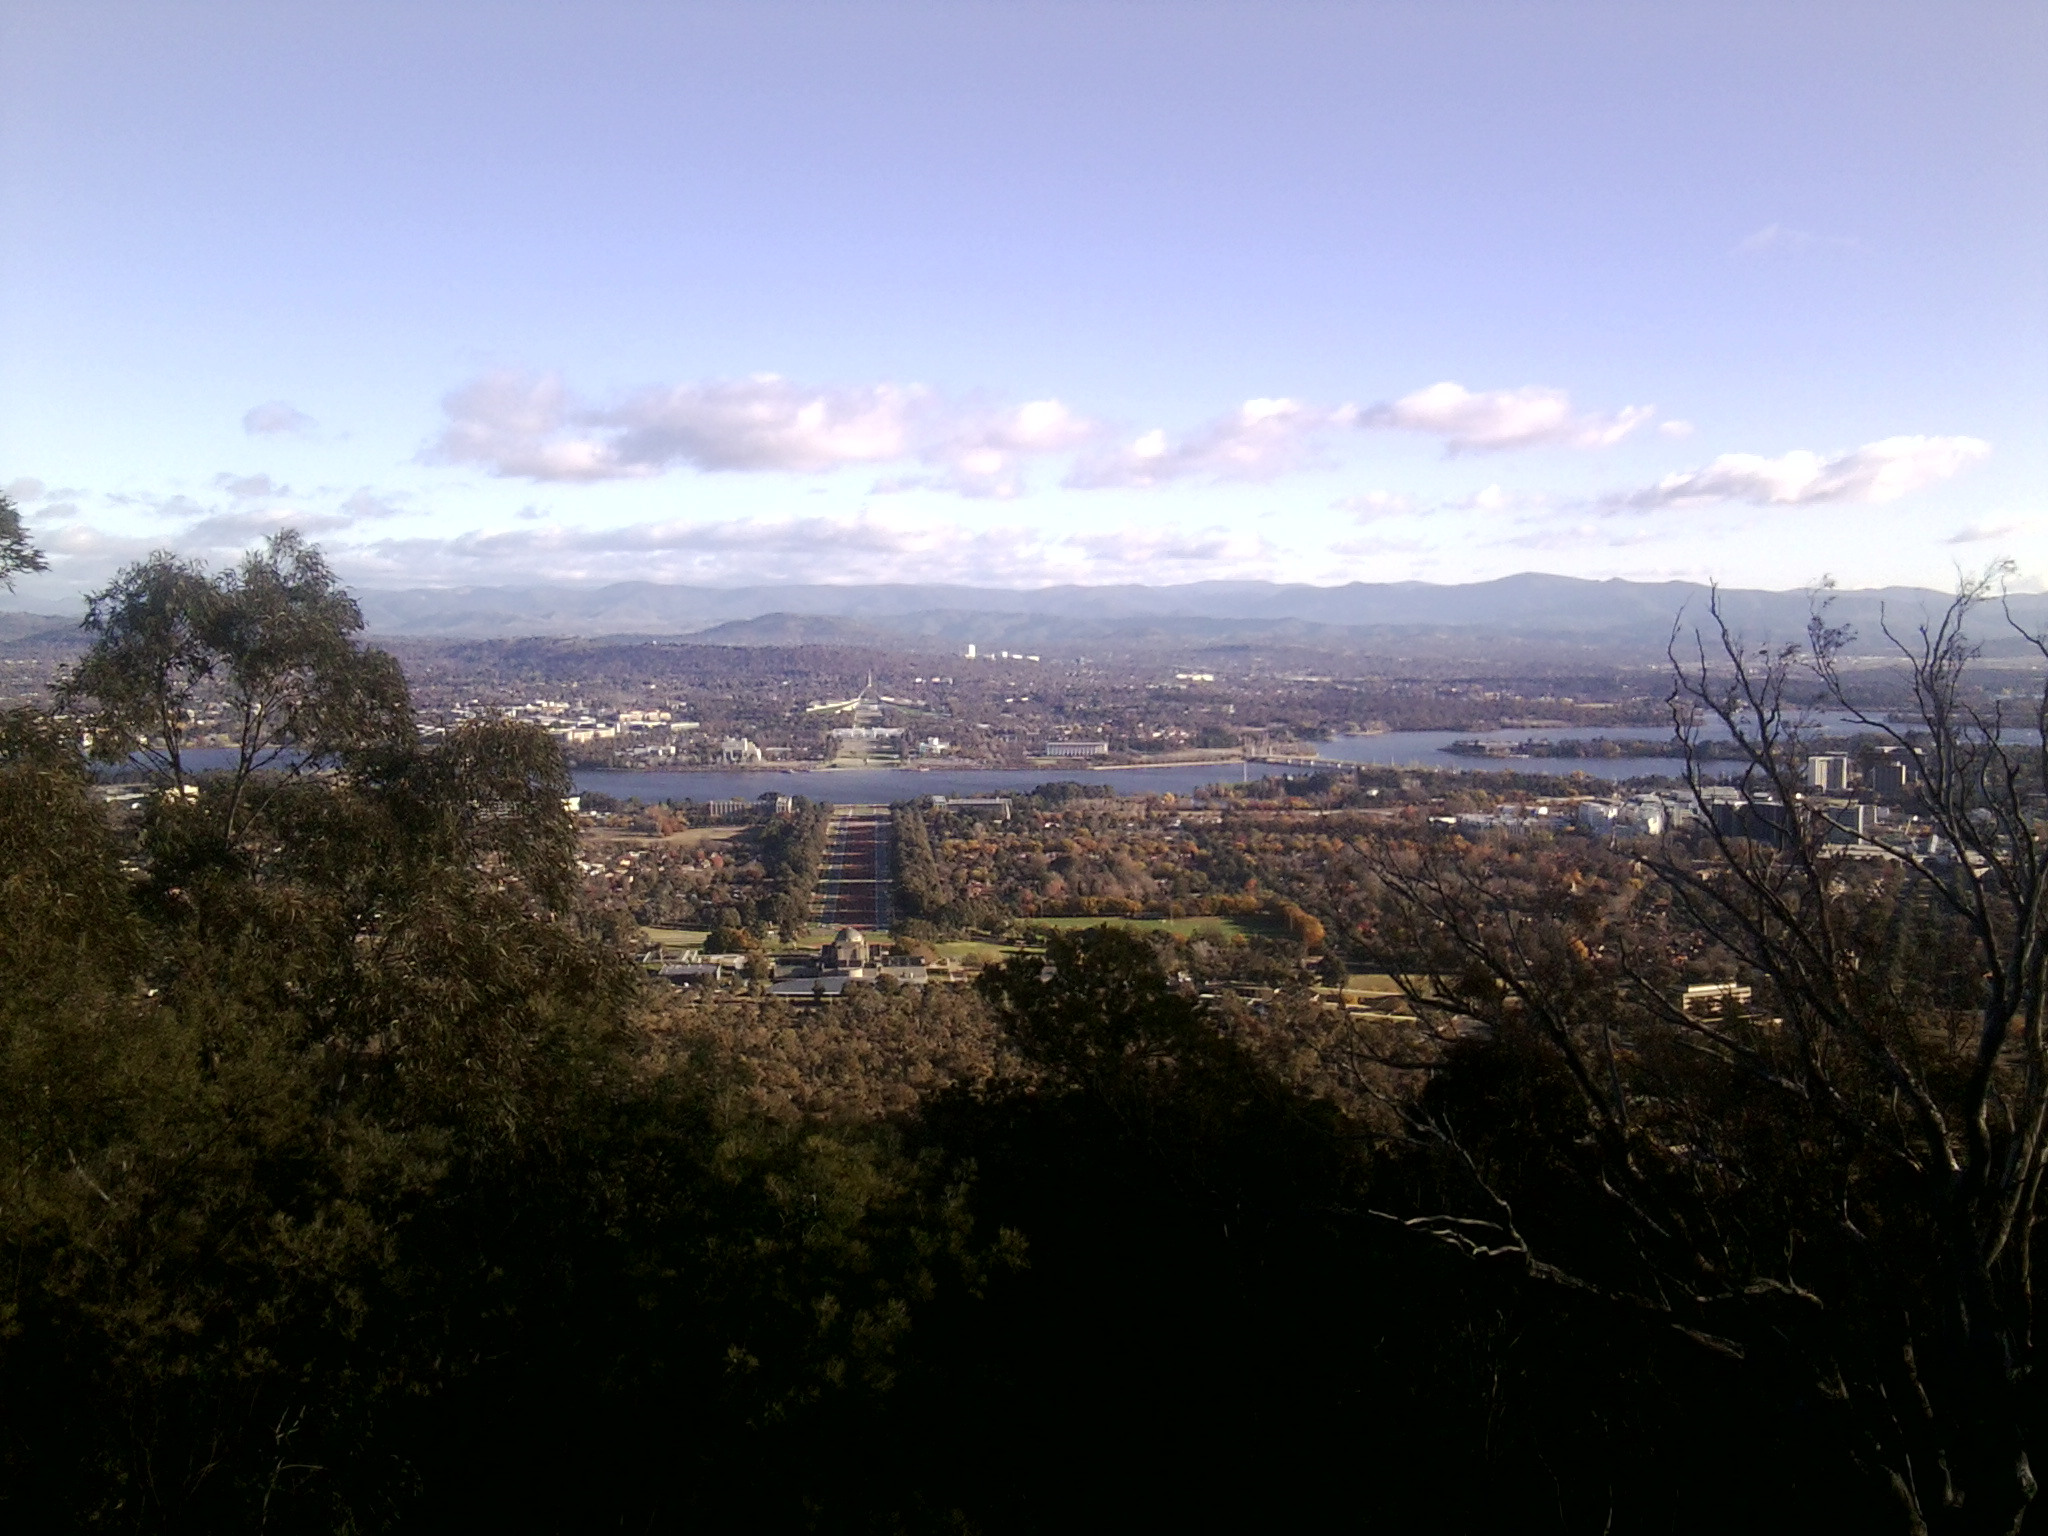
\includegraphics[scale=0.13]{location.jpg}
\end{center}
}

\subsection{Deux types de prouveurs}
\frame{\frametitle{Deux façon différentes de démontrer des théorèmes} 

\noindent \begin{tabularx}{\textwidth}{ |c|X|X| }
  \hline
  & Prouveur interactif & Prouveur automatique\\
  \hline  
  Prouveurs & HOL4, Coq, \ldots 
  & Beagle, SPASS, \ldots \\
  \hline  Expressivité & Ordre supérieur. & Premier ordre.
  \\  
  \hline Efficacité & Guidé. & Automatique. \\
  \hline Sûreté & Petit noyau.
 & Code assez long. \\
  \hline
\end{tabularx}
}

\begin{frame}
\begin{multicols}{2}
  \tableofcontents
\end{multicols}
\end{frame}

\subsection{Enoncé du problème} 
\frame{\frametitle{Enoncé du problème} 

\textit{Problème} 
Voilà deux prouveurs internes à HOL4.
\begin{enumerate}
\item[-] Metis: ordre supérieur
\item[-] Cooper: arithmétique
\end{enumerate}
\pause
\textit{Solution} Un prouveur externe.
 \begin{enumerate}
  \item[-] Beagle: premier ordre et arithmétique 
\end{enumerate}
}

\subsection{BEAGLE$\_$TAC}
\frame{\frametitle{BEAGLE$\_$TAC} 
\begin{tikzpicture}[node distance = 2cm, auto]
  % Place nodes
  \node [cloud] (conjecture) {conjecture};
  \node [block, right of=conjecture,  node distance=3cm] (HOL1) 
  {traduction};
  \node [block, right of=HOL1, node distance=3cm] (TFF1) 
  {fichier du problème};
  \node [block, right of=TFF1, node distance=3cm, yshift=-0.7cm] (Beagle) 
  {Preuve automatique};
  \node [block, below of=TFF1, node distance=2cm] (TFF2) 
  {fichier de la preuve};  
  \node [block, below of=HOL1, node distance=2cm] (HOL2) 
  {construction de la preuve};
  \node [cloud, below of=conjecture, node distance=2cm] (theorem) 
  {théorème};
  \node [label=HOL4, draw=black, ultra thick, 
  fit=(conjecture) (theorem) (HOL1) (HOL2)] {}; 
  \node [label=TFF format interface, draw=black, ultra thick, fit=(TFF1) (TFF2)] 
  {}; 
  \node [label=Beagle, draw=black, ultra thick, fit=(Beagle)] {}; 
  % Draw edges
  \draw [-to,black,ultra thick] (conjecture) -- (HOL1);
  \draw [-to,black,ultra thick] (HOL1) -- (TFF1);
  \draw [-to,,black,ultra thick] (TFF1) -- (Beagle);
  \draw [-to,black,ultra thick] (Beagle) -- (TFF2);
  \draw [-to,black,ultra thick] (TFF2) -- (HOL2);
  \draw [-to,black,ultra thick,dashed] (HOL2) -- (theorem);
\end{tikzpicture}
}

\frame{\frametitle{Les avantages du format TFF(TPTP)}

Voici une courte description du format TFF:
\begin{enumerate}
\item [-] Utilisation: répandu
\item [-] Formules: arithmétiques typées du premier ordre.
\end{enumerate}
Ses avantages sont:
\begin{enumerate}
\item [-] Lisible par un humain
\item [-] Lisible par d'autres prouveurs automatiques
\end{enumerate}
}

\subsection{HOL4} 
\frame{\frametitle{HOL4}
Voici les caractéristiques de HOL4:
\begin{enumerate}
\item [-] Prouveur interactif 
\item [-] Logique: ordre supérieur et types polymorphes
\item [-] Language: écrit en SML
\item [-] Sûreté: type [thm] abstrait
\end{enumerate} 
}

\begin{frame}[fragile]
\frametitle{Une preuve facile}

\begin{prooftree}
\AxiomC{$A \vdash A$}
\AxiomC{$B \vdash B$}
\RightLabel{$\wedge_i$}
\BinaryInfC{$A,B \vdash A \wedge B$}
\RightLabel{$\Rightarrow_i$}
\UnaryInfC{$A \vdash B \Rightarrow (A \wedge B) $}
\RightLabel{$\Rightarrow_i$}
\UnaryInfC{$\vdash A \Rightarrow (B \Rightarrow (A \wedge B)) $}
\end{prooftree}

\scriptsize
\begin{Verbatim}[frame=single]
(* forward proof *)
val th1 = ASSUME ``A:bool``;
val th2 = ASSUME ``B:bool``;
val th3 = CONJ th1 th2;
val th4 = DISCH ``B:bool`` th3;
val th5 = DISCH ``A:bool`` th4;
\end{Verbatim} 
\begin{Verbatim}[frame=single]
(* backward proof *)
g(`A ==> B ==> A /\ B `);
e(DISCH_TAC);
e(DISCH_TAC);
e(CONJ_TAC);
e(ACCEPT_TAC th1);
e(ACCEPT_TAC th2);
\end{Verbatim} 
\normalsize
\end{frame}

\subsection{Beagle}
\frame{\frametitle{Beagle}
Voici les caractéristiques de Beagle:
\begin{enumerate}
  \item [-] Prouveur automatique
  \item [-] Logique: premier ordre et types monomorphes
  \item [-] Raisonnement: premier ordre et arithmétique
  \item [-] Réponse: insatisfaisable, satisfaisable ou inconnu
\end{enumerate}
}

\frame{\frametitle{Une preuve par saturation}

\begin{tikzpicture}[auto]
  % Place nodes
  \node [cloud] (NCS) {nouvel ensemble};
  \node [cloud, above of=NCS, node distance = 1.8cm] (init) {fichier TFF};
  \node [label = below:2, cloud, below of=NCS, node distance = 2cm] (OCS) {ancien ensemble};
  % Draw edges
  \draw[-to,black,ultra thick] (NCS.east) to [out=0,in=0] node[name=down]{1} (OCS.east) ;
  \draw[-to,black,ultra thick] (OCS.west) to [out=180,in=180] node[name=up]{3} (NCS.west)  ;
  \draw[-to,black,ultra thick] (init) -- node[name=what]{parsing et normalisation} (NCS)  ;  
  % Place boxes
  \node [block, right of=down, node distance=1.5cm] (rightbox)  
  {Transfère une clause};  
  \node [block, below of=OCS, node distance=2cm] (downbox)  
  {Applique les règles possibles};      
  \node [block, left of=up, node distance=1.5cm] (leftbox)  
  {Transfère les clauses créées};   
\end{tikzpicture}
}


\section{Traduction vers le premier ordre}

\frame{\frametitle{Ordre de la traduction vers le premier ordre}
Voici les étapes de la traduction: 
\begin{enumerate}
  \item {\color{blue} Monomorphisation}
  \item Négation de la conclusion (Preuve par l'absurde)
  \item Mise en forme normale conjonctive (Arrive plusieurs fois)
  \item {\color{blue} $\lambda$-lifting}
  \item {\color{blue} Elimination des booléens}
  \item Mise sous forme d'un ensemble de clauses
  \item {\color{blue} Défonctionnalisation}
  \item Injection dans les entiers
  \item Instantiation des variables booléennes quantifiées
\end{enumerate}
}


\subsection{Monomorphisation}
\frame{\frametitle{Motivation}
Instanciation des types polymorphes de HOL4 par des types monomorphes. 
 \begin{exampleblock}{Problème}
 Théorème: $\forall x:a.\ {\color{red}C}\ x\  x$
 \\ Conjecture: ${\color{orange}C}\ 42\ 42$
 \end{exampleblock}
Unification du type des constantes  ${\color{red}C} : a \rightarrow a \rightarrow bool$  et ${\color{orange}C}: num \rightarrow num \rightarrow bool$ 
 \begin{exampleblock}{Nouveau problème}
 Théorème: $\forall x:num.\ C\ x\ x$
 \\Conjecture: $C\ 42\ 42$
\end{exampleblock}
}

\frame{\frametitle{Graphe de dépendance}
\begin{exampleblock}{Problème}
Théorème 1: $\forall x:a.\ C\ x \Rightarrow D\ x$
\\Théorème 2: $\forall x:b.\ C\ x$
\\Conjecture : $D\ 42$
\end{exampleblock}

\begin{center}
\begin{tikzpicture}[node distance = 3cm, auto]
  \node [cloud, fill=white,node distance = 3cm] (c11) {C: a};
  \node [cloud, fill=white, right of=c11,node distance = 4cm] (c12) {D: a};
  \node [cloud, fill=white, below of=c11,node distance = 1.5cm] (c21) {C: b};
  \node [cloud, fill=white, below of=c12,node distance = 3cm] (c32) {D: num};
  \draw[-to,blue,ultra thick](c11) -- (c21);
  \draw [-to,blue,ultra thick] (c21) -- (c11);
  \draw [-to,blue,ultra thick] (c12) -- (c32);
  \draw [green,ultra thick] (c11) -- (c12);
\end{tikzpicture}
\end{center}
}

\frame{\frametitle{Exemple 1: Une co-instanciation}
La flèche de substitution à droite induit une co-instanciation des constantes du premier théorème:

\begin{center}
\begin{tikzpicture}[node distance = 3cm, auto]
  \node [cloud, fill=white,node distance = 3cm] (c11) {C: a,{\color{red} num}};
  \node [cloud, fill=white, right of=c11,node distance = 4cm] (c12) {D: a,{\color{red} num}};
  \node [cloud, fill=white, below of=c11,node distance = 1.5cm] (c21) {C: b};
  \node [cloud, fill=white, below of=c12,node distance = 3cm] (c32) {D: num};
  \draw[-to,blue,ultra thick](c11) -- (c21);
  \draw [-to,blue,ultra thick] (c21) -- (c11);
  \draw [-to,blue,ultra thick] (c12) -- (c32);
  \draw [green,ultra thick] (c11) -- (c12);
\end{tikzpicture}
\end{center}
}



\frame{\frametitle{Exemple 1: Toutes les co-instanciations en parallèles}
Nous nommerons $\mathcal{T}$ cette transformation du graphe.
\begin{center}
\begin{tikzpicture}[node distance = 3cm, auto]
  \node [cloud, fill=white,node distance = 3cm] 
  (c11) {C: a,{\color{red} b},{\color{red}num}};
  \node [cloud, fill=white, right of=c11,node distance = 4cm] (c12) {D: a,{\color{red} b},{\color{red}num}};
  \node [cloud, fill=white, below of=c11,node distance = 1.5cm] (c21) {C: {\color{red} a},b};
  \node [cloud, fill=white, below of=c12,node distance = 3cm] (c32) {D: num};
  \draw [-to,blue,ultra thick] (c21) -- (c11);
  \draw [green,ultra thick] (c11) -- (c12);
\end{tikzpicture}
\end{center}
}

\frame{\frametitle{Exemple 1: Répétition des co-instanciations}
La transformation $\mathcal{T}$ précédente peut être répétée sur le nouveau graphe de dépendance que nous avons obtenu.

\begin{center}
\begin{tikzpicture}[node distance = 3cm, auto]
  \node [cloud, fill=white,node distance = 3cm] 
  (c11) {C: a,{\color{red} b},{\color{red}num}};
  \node [cloud, fill=white, right of=c11,node distance = 4cm] (c12) {D: a,{\color{red} b},{\color{red}num}};
  \node [cloud, fill=white, below of=c11,node distance = 1.5cm] (c21) {C: {\color{red} a},b,{\color{orange} num}};
  \node [cloud, fill=white, below of=c12,node distance = 3cm] (c32) {D: num};
  \draw [green,ultra thick] (c11) -- (c12);
\end{tikzpicture}
\end{center}
Ce graphe est un point fixe pour $\mathcal{T}$.
}

\frame{\frametitle{Exemple 2: Un exemple sans point fixe}
Recommençons avec un autre graphe.

\begin{center}
\begin{tikzpicture}[node distance = 3cm, auto]
  \node [cloud, fill=white,node distance = 3cm] (c11) 
  {C: a};
  \node [cloud, fill=white, right of=c11,node distance = 5.4cm] (c12) 
  {D: a$\rightarrow$n};
  \node [cloud, fill=white, below of=c11,node distance = 2cm] (c21) 
  {C: a$\rightarrow$n};
  \node [cloud, fill=white, below of=c12,node distance = 2cm] (c22) 
  {D: a};
  \draw [-to,blue,ultra thick] (c11) -- (c21);
  \draw [-to,blue,ultra thick] (c22) -- (c12);
  \draw [green,ultra thick] (c11) -- (c12);
  \draw [green,ultra thick] (c21) -- (c22);
\end{tikzpicture}
\end{center}
}

\frame{\frametitle{Exemple 2: Un exemple sans point fixe}
\begin{center}
\begin{tikzpicture}[node distance = 3cm, auto]
  \node [cloud, fill=white,node distance = 3cm] (c11) 
  {C: a,{\color{red} a$\rightarrow$n}};
  \node [cloud, fill=white, right of=c11,node distance = 5.4cm] (c12) 
  {D: a$\rightarrow$n,{\color{red}(a$\rightarrow$n)$\rightarrow$n}};
  \node [cloud, fill=white, below of=c11,node distance = 2cm] (c21) 
  {C: a$\rightarrow$n,{\color{red}(a$\rightarrow$n)$\rightarrow$n}};
  \node [cloud, fill=white, below of=c12,node distance = 2cm] (c22) 
  {D: a,{\color{red} a$\rightarrow$n}};
  \draw [-to,blue,ultra thick] (c11) -- (c21);
  \draw [-to,blue,ultra thick] (c22) -- (c12);
  \draw [green,ultra thick] (c11) -- (c12);
  \draw [green,ultra thick] (c21) -- (c22);
\end{tikzpicture}
\end{center}
}



\frame{\frametitle{Exemple 2: Un exemple sans point fixe}
\begin{center}
\scriptsize
\begin{tikzpicture}[scale = 0.5]
  \node [cloud, fill=white] (c11) 
  {C:a,{\color{red} a$\rightarrow$n},{\color{orange}(a$\rightarrow$n)$\rightarrow$n}};
  \node [cloud, fill=white,right of=c11,node distance = 5.4cm] (c12) 
  {D:a$\rightarrow$n,{\color{red}
  (a$\rightarrow$n)$\rightarrow$n},{\color{orange}
  ((a$\rightarrow$n)$\rightarrow$n)$\rightarrow$n}
  };
  \node [cloud,  fill=white, below of=c11, xshift=1cm, node distance = 2cm] (c21) 
  {C:a$\rightarrow$n,{\color{red}
  (a$\rightarrow$n)$\rightarrow$n},{\color{orange}
  ((a$\rightarrow$n)$\rightarrow$n)$\rightarrow$n}
  };
  \node [cloud, fill=white, right of=c21 ,node distance = 5.4cm] (c22) 
  {D:a,{\color{red} a$\rightarrow$n},{\color{orange}
  (a$\rightarrow$n)$\rightarrow$n}};
  \draw [-to,blue,ultra thick] (c11) -- (c21);
  \draw [-to,blue,ultra thick] (c22) -- (c12);
  \draw [green,ultra thick] (c11) -- (c12);
  \draw [green,ultra thick] (c21) -- (c22);
\end{tikzpicture}
\normalsize
\end{center}
La transformation $\mathcal{T}$ ne trouve pas de point fixe.
}


\frame{\frametitle{Instanciation des théorèmes données par l'utilisateur}
\begin{enumerate}
\item Terminaison: un point fixe ou une borne arbitraire
\item Extraction d'un ensemble de substitutions pour chaque théorème
\begin{center}
\begin{tikzpicture}[node distance = 3cm, auto]
  \node [cloud, fill=white,node distance = 3cm] 
  (c11) {C: a,{\color{red} b},{\color{red}num}};
  \node [cloud, fill=white, right of=c11,node distance = 4cm] (c12) {D: a,{\color{red} b},{\color{red}num}};
  \node [cloud, fill=white, below of=c11,node distance = 1.5cm] (c21) {C: {\color{red} a},b,{\color{orange} num}};
  \node [cloud, fill=white, below of=c12,node distance = 3cm] (c32) {D: num};
  \draw [green,ultra thick] (c11) -- (c12);
\end{tikzpicture}
\end{center}
\item Instanciation
\end{enumerate}
}

\subsection{Autres étapes}

\frame{\frametitle{Ordre de la traduction vers le premier ordre}
Voici les étapes de la traduction: 
\begin{enumerate}
  \item {\color{blue} Monomorphisation}
  \item Négation de la conclusion (Preuve par l'absurde)
  \item Mise en forme normale conjonctive (Arrive plusieurs fois)
  \item {\color{blue} $\lambda$-lifting}
  \item {\color{blue} Elimination des booléens}
  \item Mise sous forme d'un ensemble de clauses
  \item {\color{blue} Défonctionnalisation}
  \item Injection dans les entiers
  \item Instantiation des variables booléennes quantifiées
\end{enumerate}
}

\frame{\frametitle{$\lambda$-lifting}
Cette étape élimine les $\lambda$-abstractions restantes.
\[ P\ (\lambda x.x+1) \]
\[ \exists g.\ (\forall x.\ g\ x = x + 1) \wedge P\ g \]
}

\frame{\frametitle{Elimination des booléens}
Supposons que la formule booléenne $!x.\ x=0$ soit l'argument d'une fonction $f$.
\[P (!x.\ x=0)\]

\[((!x.\ x=0) \Rightarrow P\ true) \wedge 
   (\neg (!x.\ x=0)  \Rightarrow P\ false)\]
}

\frame{\frametitle{Défonctionnalisation}

Soit $App$ vérifiant $App\ f\ x$ = $f\ x$. On effectue une défonctionnalisation lorsqu'une fonction non-arithmétique: 

 \begin{enumerate}
 \item [-] est quantifiée
   \[!h.\ h\ x\ y = 0\]
   \[!h.\ App\ (App\ h\ x)\ y = 0\]
 \item [-] a le même type qu'une fonction quantifiée
 \item [-] a un nombre d'arguments qui varie
   \[h\ x\ y\ z\wedge h\ x = g\]
   \[App\ (App\ (h\ x)\ y)\ z \wedge h\ x = g\]
 \end{enumerate}.
}



\frame{\frametitle{Résultats avec monomorphisation}
Nombre total de problèmes: 271
\begin{center}

\end{center}
}

\frame{\frametitle{Utilisation des différentes parties de la traduction}

\begin{center}
\begin{tikzpicture}[scale=0.8]
\begin{axis}[ybar,enlargelimits=0.15,legend style={at={(2,2)},anchor=north,legend columns=0},ylabel={nombre de problèmes},symbolic x coords={monomorphisation,point fixe,lambda-lifting,booleen,naturels,ordre superieur,preuve},xtick=data,
nodes near coords,
nodes near coords align={vertical},
x tick label style={rotate=45,anchor=east},]
\addplot coordinates {(monomorphisation,139) (point fixe,112) (lambda-lifting,60) (booleen,72)(naturels,162)(ordre superieur,86)(preuve,271)};
\end{axis}
\end{tikzpicture}
\end{center}
}

\frame{\frametitle{Résultats sur des problèmes arithmétiques}
Nombre de problèmes: 65. 
\\Dans ces problèmes, tous les théorèmes (79) ne concernant que l'arithmétique ont été effacés. 
\begin{center}
\begin{tikzpicture}[scale=2.5]
\newcounter{a}
\newcounter{b}

\setcounter{a}{\value{b}}
    \addtocounter{b}{88}
    \slice{\thea/100*360}
          {\theb/100*360}
          {88\%}{insatisfaisable}{green}

\setcounter{a}{\value{b}}
    \addtocounter{b}{9}
    \slice{\thea/100*360}
          {\theb/100*360}
          {9\%}{inconnu}{red}

\setcounter{a}{\value{b}}
    \addtocounter{b}{3}
    \slice{\thea/100*360}
          {\theb/100*360}
          {3\%}{time out}{red}
\end{tikzpicture}
\end{center}
}

\section{Rejouage de la preuve}
\frame{\frametitle{Principe général}
\begin{tikzpicture}[node distance = 2cm, auto]
  % Place nodes
  \node [cloud] (conjecture) {conjecture};
  \node [block, right of=conjecture,  node distance=3cm] (HOL1) 
  {traduction (premier ordre)};
  \node [block, right of=HOL1, node distance=3cm] (TFF1) 
  {fichier du problème};
  \node [block, right of=TFF1, node distance=3cm, yshift=-0.7cm] (Beagle) 
  {Preuve automatique};
  \node [block, below of=TFF1, node distance=2cm] (TFF2) 
  {fichier de la preuve};  
  \node [block, below of=HOL1, node distance=2cm] (HOL2) 
  {construction de la preuve};
  \node [cloud, below of=conjecture, node distance=2cm] (theorem) 
  {théorème};
  \node [label=HOL4, draw=black, ultra thick, 
  fit=(conjecture) (theorem) (HOL1) (HOL2)] {}; 
  \node [label=TFF format interface, draw=black, ultra thick, fit=(TFF1) (TFF2)] 
  {}; 
  \node [label=Beagle, draw=black, ultra thick, fit=(Beagle)] {}; 
  % Draw edges
  \draw [-to,black,ultra thick] (conjecture) -- (HOL1);
  \draw [-to,black,ultra thick] (HOL1) -- (TFF1);
  \draw [-to,,black,ultra thick] (TFF1) -- (Beagle);
  \draw [-to,black,ultra thick] (Beagle) -- (TFF2);
  \draw [-to,black,ultra thick] (TFF2) -- (HOL2);
  \draw [-to,black,ultra thick,dashed] (HOL2) -- (theorem);
\end{tikzpicture}
}

\subsection{Extraction d'une preuve}
\frame{\frametitle{Extraction d'une preuve}
\begin{tikzpicture}[auto]
  % Place nodes
  \node [cloud] (NCS) {nouvel ensemble};
  \node [cloud, fill=white, above of=NCS, node distance = 1.5cm] (init) {fichier TFF};
  \node [label = 2, cloud, below of=NCS, node distance = 2cm] (OCS) {ancien ensemble};
  % Draw edges
  \draw[-to,black,ultra thick] (NCS.east) to [out=0,in=0] node[name=down]{1} (OCS.east) ;
  \draw[-to,black,ultra thick] (OCS.west) to [out=180,in=180] node[name=up]{3} (NCS.west)  ;
  \draw[-to,black,ultra thick] (init) -- node[name=what]{parsing et normalisation} (NCS)  ;
  % Place boxes
  \node [block, right of=down, node distance=1.5cm] (rightbox)
  {Transfère une clause};
  \node [block, below of=OCS, node distance=1.5cm] (downbox)
  {Applique les règles possibles};
  \node [block, left of=up, node distance=1.5cm] (leftbox)
  {Transfère les clauses créées};
  \node [cloud, fill=white, below of=rightbox, node distance=2.5cm] (trace){fichier trace};
  \draw [-to,black,ultra thick] (down.west) to [out=270,in=90] (trace)  ;
\end{tikzpicture}
}

\subsection{Construction de la preuve}
\frame{\frametitle{Construction de la preuve}
\begin{enumerate}
\item [-] Lecture de la preuve: utilise des dictionnaires de variables et de types 

\item [-] Rejouage de la preuve: chaque étape peut être résolue par metis, cooper ou une combinaison des deux. (en théorie!!) 
\end{enumerate}
}

\section{Conclusion}

\subsection{Résumé}
\frame{\frametitle{Qualités et limites de l'interaction HOL4-Beagle}
Qualités: 
\begin{enumerate}
\item [-] Résout des problèmes arithmétiques sans guidage
\item [-] Un format de communication répandu
\item [-] Une traduction correcte préservant l'insatisfaisabilité
\end{enumerate} 
Limites: 
\begin{enumerate}
\item [-] 20\% des conjectures non prouvées par Beagle 
\item [-] Echec du rejouage de la preuve dans beaucoup de cas 
\item [-] Une traduction incomplète
\item [-] Une traduction ne préservant pas la satisfaisabilité
\end{enumerate} 
}

\subsection{Perspectives}
\frame{\frametitle{Améliorations possibles de la traduction}

\begin{enumerate}
\item [-] Traduire les rationnels et les réels
\item [-] Générer automatiquement des théorèmes aidant à prouver la conjecture
\item [-] Normalisation des formules arithmétiques dans les preuves.
 \[x < y + 1 + 2 \longrightarrow x - y < 3\]
\end{enumerate}
}



\end{document}

